\documentclass[a4paper,12pt, oneside]{book}

% \usepackage{fullpage}
\usepackage[italian]{babel}
\usepackage[utf8]{inputenc}
\usepackage{amssymb}
\usepackage{amsthm}
\usepackage{graphics}
\usepackage{amsfonts}
\usepackage{listings}
\usepackage{amsmath}
\usepackage{amstext}
\usepackage{engrec}
\usepackage{rotating}
\usepackage{verbatim}
\usepackage[safe,extra]{tipa}
%\usepackage{showkeys}
\usepackage{multirow}
\usepackage{hyperref}
\usepackage{microtype}
\usepackage{fontspec}
\usepackage{enumerate}
\usepackage{braket}
\usepackage{marginnote}
\usepackage{pgfplots}
\usepackage{cancel}
\usepackage{polynom}
\usepackage{booktabs}
\usepackage{enumitem}
\usepackage{framed}
\usepackage{pdfpages}
\usepackage{pgfplots}
\usepackage{algorithm}
% \usepackage{algpseudocode}
\usepackage[cache=false]{minted}
\usepackage{mathtools}
\usepackage[noend]{algpseudocode}

\usepackage{tikz}\usetikzlibrary{er}\tikzset{multi  attribute /.style={attribute
    ,double  distance =1.5pt}}\tikzset{derived  attribute /.style={attribute
    ,dashed}}\tikzset{total /.style={double  distance =1.5pt}}\tikzset{every
  entity /.style={draw=orange , fill=orange!20}}\tikzset{every  attribute
  /.style={draw=MediumPurple1, fill=MediumPurple1!20}}\tikzset{every
  relationship /.style={draw=Chartreuse2,
    fill=Chartreuse2!20}}\newcommand{\key}[1]{\underline{#1}}
  \usetikzlibrary{arrows.meta}
  \usetikzlibrary{decorations.markings}
  \usetikzlibrary{arrows,shapes,backgrounds,petri}
\tikzset{
  place/.style={
        circle,
        thick,
        draw=black,
        minimum size=6mm,
    },
  transition/.style={
    rectangle,
    thick,
    fill=black,
    minimum width=8mm,
    inner ysep=2pt
  },
  transitionv/.style={
    rectangle,
    thick,
    fill=black,
    minimum height=8mm,
    inner xsep=2pt
    }
  } 
\usetikzlibrary{automata,positioning}
\usepackage{fancyhdr}
\pagestyle{fancy}
\fancyhead[LE,RO]{\slshape \rightmark}
\fancyhead[LO,RE]{\slshape \leftmark}
\fancyfoot[C]{\thepage}
\usepackage[usenames,dvipsnames]{pstricks}
\usepackage{epsfig}
\usepackage{pst-grad} % For gradients
\usepackage{pst-plot} % For axes
\usepackage[space]{grffile} % For spaces in paths
\usepackage{etoolbox} % For spaces in paths
\makeatletter % For spaces in paths
\patchcmd\Gread@eps{\@inputcheck#1 }{\@inputcheck"#1"\relax}{}{}
\makeatother

\title{Teoria della Computazione}
\author{UniShare\\\\Davide Cozzi\\\href{https://t.me/dlcgold}{@dlcgold}}
\date{}

\pgfplotsset{compat=1.13}
\begin{document}
\maketitle

\definecolor{shadecolor}{gray}{0.80}
\setlist{leftmargin = 2cm}
\newtheorem{teorema}{Teorema}
\newtheorem{definizione}{Definizione}
\newtheorem{esempio}{Esempio}
\newtheorem{corollario}{Corollario}
\newtheorem{lemma}{Lemma}
\newtheorem{osservazione}{Osservazione}
\newtheorem{nota}{Nota}
\newtheorem{esercizio}{Esercizio}
\algdef{SE}[DOWHILE]{Do}{doWhile}{\algorithmicdo}[1]{\algorithmicwhile\ #1}
\tableofcontents
\renewcommand{\chaptermark}[1]{%
  \markboth{\chaptername
    \ \thechapter.\ #1}{}}
\renewcommand{\sectionmark}[1]{\markright{\thesection.\ #1}}
\newcommand{\floor}[1]{\lfloor #1 \rfloor}
\newcommand{\MYhref}[3][blue]{\href{#2}{\color{#1}{#3}}}%
\chapter{Introduzione}
\textbf{Questi appunti sono presi a lezione. Per quanto sia stata fatta
  una revisione è altamente probabile (praticamente certo) che possano
  contenere errori, sia di stampa che di vero e proprio contenuto. Per
  eventuali proposte di correzione effettuare una pull request. Link: }
\url{https://github.com/dlcgold/Appunti}.\\
\chapter{Prerequisiti di computazione}
L'informatica è costruita su una logica matematica. Il punto di partenza è stato
dettato da Turing (con la \textbf{macchina di Turing} (\textit{TM})) e questo
pensiero si è poi sviluppato nel tempo. Turing, con la sua macchina logica, ha
dimostrato che ci sono funzioni non calcolabili, verità logiche non
dimostrabili.\\ Subito dopo la macchina di Turing nasce la teoria della
\textbf{complessità   computazionale}, col fine di classificare il problemi in
base alla difficoltà delle soluzioni mediante macchine di calcolo. Tale
\textit{difficoltà} viene stimata rispetto a \textbf{spazio e tempo}. La teoria
della \textbf{complessità computazionale} si riferisce a varie \textbf{classi
  di complessità} che 
classificano, in un primo approccio, \textit{problemi decisionali} descritti da
funzioni binarie che hanno in input una stringa sull'alfabeto $\{0,1\}$ e
restituiscono un bit (o 0 o 1). Questo perché le macchine di Turing ragionano in
binario. Si ha quindi:
\[f:\{0,1\}^*\to {0,1}\]
\textbf{Esistono problemi che si è dimostrato non essere risolvibili in tempo
  efficiente.}\\
Tra le classi abbiamo i \textbf{problemi NP} e \textbf{problemi P}. Inoltre i
problemi NP sono a loro volta classificabili tra loro cercando i più difficili,
ottenendo \textbf{problemi NP-hard} e \textbf{problemi NP-complete} (esistono
varie dimostrazioni per la \textit{NP-completezza}).
\section{Tempo di calcolo di una TM}
\begin{definizione}
  Sia $T:\mathbb{N}\to \mathbb{N}$ una funzione calcolabile da TM e $L\pi$ un
  linguaggio di decisione (dove $\pi$ sta per ``problema'' e ``di decisione'' ci
  ricorda che il risultato sarà binario) allora una \textbf{TM deterministica}
  $M$ accetta L$\pi$ in tempo $T(n)$ se, $\forall x\in L\pi$, con $|x|=n$, $M$
  accetta $x$ in $T(n)$ mosse o configurazioni
\end{definizione}
\begin{definizione}
  Un \textbf{problema di decisione} $\pi$ riceve in input un'istanza $x$ e
  l'output è:
  \begin{itemize}
    \item 0 che vuole dire \textit{no}
    \item 1 che vuole dire \textit{yes}
  \end{itemize}
  Un linguaggio $L\pi$ restituisce 1 per tutti gli $x$ che appartengono al
  linguaggio. Quindi $L\pi$ è l'insieme degli input di $\pi$ su cui l'output è
  1 (è l'analogo della \emph{funzione caratteristica} di un insieme, ovvero la
  funzione che risponde 1 sse un certo elemento appartiene all'insieme di
  riferimento).\\
  La \textbf{funzione associata al problema} si chiama $f\pi$ ed è la funzione
  che dato un input restituisce 1 sse l'input appartiene al $L\pi$.
\end{definizione}
Approfondiamo ora lo studio della \textbf{classe P}.
\begin{definizione}
  La classe dei linguaggi di decisione accettati in tempo
  $T(n)=cn^p,\,p\in\mathbb{N},\, p\neq 0$ da una TM deterministica è detta
  \textbf{classe P}, quindi in un tempo polinomiale sulla dimensione dell'input
  $n$, è detta \textbf{classe P}. Quindi P è una classe di \textbf{problemi di
    decisione}. \\
  Potenzialmente $p$ potrebbe anche non essere un intero in quanto si potrebbero
  avere tempi frazionari.
\end{definizione}
\begin{definizione}
  Si definisce che $L\pi$ è accettato da una TM in tempo $T(n)$ se $\exists
  \,\,T :\mathbb{N}\to \mathbb{N}$ calcolabile da TM e $\forall x\in L\pi$, con
  $|x|=n$, la TM accetta $x$ e risponde 1 (\textit{yes}) in al più $T(n)$ mosse
  di calcolo (dette anche configurazioni).\\
  Nel caso del modello della macchina RAM si ha la stessa situazione con però
  $T(n)$ \textbf{istruzioni RAM} e si dice che $L\pi$ è accettato dalla macchina
  RAM (si può dire che è anche deciso dell'algoritmo A della macchina RAM). In
  caso contrario la macchina RAM restituisce \textit{no}, in quanto si parla di
  ``decisione'' oltre che di ``accettazione'' (a differenza della TM, dove però
  si può ottenere lo stesso discorso parlando di TM complementare $M'$, che in
  $T(n)$ mi risponderà yes alla richiesta che un input non appartenga a
  $L\pi$, altrimenti bisogna fissare un limite di tempo per ottenere yes).\\
  È dimostrabile che se $L\pi$ è accettabile in tempo polinomiale allora nello
  stesso tempo è anche decidibile.\\
  La differenza tra accettazione e decisione sarà fondamentale nel
  \textbf{modello non deterministico}.
\end{definizione}
\begin{shaded}
  Si ricordi che il \textbf{modello RAM (\textit{Random Access Machine})} è
  usato per studiare il tempo di calcolo di 
  uno pseudocodice. È un modello teorico (una macchina teorica ``simile'' a
  quelle reali) dotato di istruzioni come
  \textit{load, store, add, etc$\ldots$} dove un codice (ipoteticamente in
  qualsiasi linguaggio incluso lo pseudocodice) viene tradotto in una sorta di
  linguaggio macchina (linguaggio RAM), dove $n$ è un intero rappresentante il
  numero di istruzioni RAM necessarie per ottenere l'output ($n$ è detto
  \textbf{tempo uniforme}). Sul linguaggio RAM si può studiare anche lo spazio
  calcolato come numero di bit necessari per la computazione (è detto
  \textbf{costo logaritmico}). In questo secondo punto il costo di
  un'istruzione, come ad esempio \textit{load(n)}, è logaritmico rispetto
  all'operando $n$ ($\,\log_2 n$), studia quindi la \emph{dimensione}
  dell'input.
\end{shaded}
Consideriamo ora un modello basato su algoritmi.
\begin{definizione}
  Sia $L\pi$ un linguaggio di decisione e $t:\mathbb{N}\to\mathbb{N}$ una
  funzione calcolabile, allora un algoritmo $A$ accetta $L\pi$ in tempo $T(n)$
  sse $\forall x\in L\pi$, con $|x|=n$, $A$ termina su input $x$ dopo $T(|x|)$
  passi di calcolo, ovvero istruzioni esguite, producendo 1 come output. Quindi
  P è la classe dei linguaggi di decisione accettati in tempo
  $T(n)=cn^p,\,p\in\mathbb{N}$ (con lo stesso discorso di sopra su $p$) da un
  algoritmo $A$ in tempo polinomiale.
\end{definizione}
\chapter{Complessità computazionale}
Si cerca di catalogare dal punto di vista computazionale i \textbf{problemi
  intrattabili}, ovvero problemi risolvibili ma non in modo \textbf{efficiente}
(ovvero in tempo polinomiale). In alcuni casi si pensa che non esista una
soluzione ma non si hanno dimostrazioni in merito mentre in altri casi è
addirittura dimostrato. Abbiamo quindi delle categorie informali per i problemi:
\begin{itemize}
  \item \textbf{facili}, so risolverli in modo efficiente. È la \textbf{classe P}
  \item \textbf{difficili} o, più formalmente, \textbf{intrattabile}, so
  risolverli ma non in modo efficiente e non ho una 
  dimostrazione che mi assicuri che non siano risolvibili in modo efficiente. È
  la \textbf{classe NP} e la sua sottoclasse \textbf{NP-complete}
  \item \textbf{dimostrabilmente difficili}, so risolverli ma so che non esiste
  un algoritmo efficiente in quanto è stato dimostrato che non può esistere
  \item \textbf{impossibili}, non so risolverli sempre neanche in modo non
  efficiente (esiste almeno un input che manda in crisi l'algoritmo ma esiste
  almeno un caso in cui funzioni)
\end{itemize}
Come formalismo useremo la \textbf{Macchina di Turing (\textit{TM})},
\textit{deterministica} e \textit{non deterministica}. Analizzeremo in primis
\textbf{problemi sui grafi}. Un grafo è definito come $G=(V,E)$, con $V$ insieme
dei vertici e $E$ insieme degli archi. Un grafo può essere \textit{orientato} o
\textit{non orientato}. Un \textbf{cammino} tra due vertici è una sequenza di
archi che mi porta da un vertice all'altro. Un cammino è detto \textbf{ciclo} se
il vertice sorgente coincide con quello di destinazione. Due vertici sono
\textbf{connessi} se esiste un cammino che li collega. Un \textbf{grafo
  connesso} è un grafo dove per ogni coppia di vertici si ha che essi sono
connessi. Se questo cammino è di un solo arco si parla di \textbf{grafo
  completo}, ovvero ogni vertice è \textbf{adiacente} ad ogni altro. Si parla di
\textbf{grafo pesato} se si ha una funzione $W$ che associa un peso ad ogni
arco. \\
Useremo anche la teoria dei linguaggi formali con $V$ alfabeto e stringhe
costruite su $V$. Con $\varepsilon$ abbiamo la stringa vuota e con $V^*$ è
l'insieme di tutte le possibili stringhe costruibili con quell'alfabeto, inclusa
la stringa vuota. $V^*$ è un insieme infinito. Con $V^+$ indico
$V^*/\varepsilon$, ovvero senza la stringa vuota. Un \textbf{linguaggio} $L$ è
un sottoinsieme di $V^*$, quindi $L\subseteq V^*$, che comprende tutti gli
elementi di $V^*$ che seguono una certa \textbf{proprietà} (o più
proprietà). Anche $L$ è un insieme infinito.\\
Un'altra nozione è quella di \textbf{problema}. Un problema computazionale è una
``questione'' a cui si cerca risposta. Più formalmente un problema è specificato
da \textbf{parametri} (l'input del problema) e le \textbf{proprietà} che deve
soddisfare la \textbf{soluzione} (l'output). L'\textbf{istanza} di un problema
specificando certi parametri in input al problema (input che devono essere
coerenti ai parametri richiesti).\\
Cominciamo con degli esempi di problemi comunque risolvibili.
\begin{esempio}
  Considero il problema \emph{arco minimo}. Come parametro ho un grafo pesato
  sugli archi $G=(V,E)$. Le proprietà della soluzione è che voglio l'arco con
  peso minimo.\\
  Per risolvere guardo tutti gli archi è vedo quello di peso minimo. Dato che
  basta iterare su tutti gli archi quindi la soluzione è in $O(n)$ (in realtà
  $\Theta(n)$), quindi in \textbf{tempo lineare} sul numero di archi (è quindi
  in \textbf{tempo polinomiale})
\end{esempio}
\begin{esempio}
  Considero il problema \emph{raggiungibilità}. Come parametro ho un grafo non
  pesato $G=(V,E)$ e due vertici, uno sorgente e uno destinazione, tali che
  $v_s,v_d\in V$. Le proprietà della soluzione è che voglio sapere se posso
  arrivare a $v_d$ partendo da $v_s$.\\
  Per risolvere studio tutti i cammini che partono da $v_s$ e posso dare la
  risposta. Una soluzione del genere è in tempo $O(2^{|E|})$. Il tempo quindi
  cresce in \textbf{modo esponenziale}. Una soluzione migliore è quella di usare
  un \textbf{algoritmo di visita} che richiede tempo $O(|V|+|E|)$, ovvero un
  \textbf{tempo polinomiale}. Quindi per quanto all'inizio si pensi
  che sia un \textbf{problema intrattabile} si scopre che è un \textbf{problema
    facile} 
\end{esempio}
\begin{esempio}
  Considero il problema \emph{TSP}. Come parametro ho un grafo pesato sugli
  archi e completo $G=(V,E)$. Le proprietà della soluzione è che voglio sapere
  il \emph{cammino minimo} (in realtà un ciclo) che tocca tutti i vertici una e
  una sola volta (una volta trovata la soluzione non mi interessa la sorgente
  essendo il grafo completo). \\
  Sarebbe facile determinare \textbf{un} ciclo ma non quello di peso minimo e
  per farlo devo trovare tutti i cicli e trovare quello di peso minimo. Ho
  quindi un algoritmo che è $O(2^n)$ (nella realtà è circa $O(n!)$ che è
  comunque esponenziale per l'\textbf{approssimazione di Stirling}). In questo
  caso non si riesce a pensare ad una soluzione che non sia esponenziale nel
  tempo (anche se per alcuni input sia di facile risoluzione, basti pensare ad
  avere tutti gli archi di peso 1, ma mi basta avere un input problematico). Non
  potendo però dimostrare che sia irrisolvibile si dice che è un
  \textbf{problema intrattabile}. \textit{TSP} è uno dei 10 problemi famosi per
  i quali ti danno un milione di dollari se dimostri che è o \emph{facile} o
  \emph{impossibile}
\end{esempio}
Per completezza definiamo un \textbf{algoritmo} come una sequenza di
\textbf{istruzioni elementari} (supportate dal calcolatore) che, eseguite in
sequenza, mi portano alla soluzione di un problema. Si ha quindi che un
algoritmo $A$ risolve un problema $\Pi$ se per ogni possibile istanza di $\Pi$
l'algoritmo $A$ mi da la risposta corretta. Distinguo però:
\begin{itemize}
  \item \textbf{algoritmo efficiente}, che mi da la soluzione in \textbf{tempo
    polinomiale} rispetto alla \textbf{dimensione dell'input}. Ho un
  \textit{caso peggiore} limitato superiormente da un \textbf{polinomiale}:
  $O(p(n))$. Ho una crescita di tempo accettabile all'aumentare
  dell'input. Diciamo comunque che è dura anche solo raggiungere $O(n^{10})$
  quindi anche se dire polinomiale potrebbe voler dire $O(n^{10000000})$ non si
  hanno casi reali di questo tipo
  \item \textbf{algoritmo non efficiente}, che mi da la soluzione ma in tempo
  superiore a quello \textbf{polinomiale}. Ho un \textit{caso peggiore} limitato
  superiormente da un \textbf{esponenziale}: $O(2^n)$. Ho una crescita di tempo
  assolutamente non accettabile (esponenziale appunto) all'aumentare dell'input 
\end{itemize}
\textit{Se ho anche solo un caso di input che porta a tempo esponenziale ho
  comunque un algoritmo non efficiente}.\\
Spesso \textbf{problemi intrattabili} vengono risolti tramite approssimazioni
per arrivare ad una soluzione accettabile anche se non la migliore ma non sempre
è possibile effettuare delle approssimazioni.\\
Anche se avessi ha che fare con un computer mille volte migliore di quelli
attuali, un problema esponenziale avrà comunque tempi non accettabili in
proporzione ad un problema polinomiale. Quindi non sarà il miglioramento
hardware a permettere di rendere accettabile la soluzione di problemi
esponenziali.\\
Un \textbf{algoritmo intrattabile} quindi non risolve in modo efficiente tutti
gli input. Bisognerà trovare un modo per capire se un algoritmo è
\textbf{intrattabile} per davvero.\\
Studiamo ora il tempo di calcolo di una \textbf{macchina di Turing non
  deterministica (\textit{NTDM})}:
\begin{definizione}
  Sia $T:\mathbb{N}\to\mathbb{N}$ una funziona calcolabile da TM. Dato $L\pi$ un
  linguaggio di decisione allora una $NDTM$ $M$. $M$ accetta $L\pi$ in tempo
  $T(n)$ se per ogni $x$ in $L\pi$ ,con $|x|=n$,  $M$ accetta $x$ in $T(n)$
  mosse (o configurazioni).\\
  Quindi la \textbf{classe NP} è la classe dei linguaggi di decisione accettati
  in tempo $T(n)=cn^p,\,\,\,p\in \mathbb{N}$ da una $NDTM$
\end{definizione}
Diamo una definizione alternativa di NP:
\begin{definizione}
  Sia $L\pi$ un linguaggio di decisione, $N:n\to n$ una funzione calcolabile,
  $y$ una stringa di lunghezza polinomiale nell'input, allora un algoritmo $A$
  con ``certificato'' accetta $L\pi$ in tempo $t(n)$ se per ogni $x$ in $L\pi$,
  con $|x|=n$, A termina su input $(x,y)$ dopo $t(|x|)$ passi di calcolo
  (istruzioni eseguite) producendo 1 in output.
  Quindi la \textbf{classe NP} è la classe dei linguaggi (o problemi) di
  decisione accettati in tempo $T(n)=cn^p,\,\,\,p\in\mathbb{N}$ da un algoritmo
  $A$ ``certificato''
\end{definizione}
Resta da capire il significato del termine ``certificato''.
\begin{definizione}
  Preso un algoritmo $A$ definiamo cosa significa che sia ``certificato'' si
  compone di un input $(x,y)$ con $y$ che è una stringa, nel dettaglio una
  \textbf{dimostrazione}, che garantisce che $x\in L\pi$.
\end{definizione}
Vediamo un esempio:
\begin{esempio}
  Uso un problema NP come esempio, quindi $\pi\in NP$, per avere un algoritmo
  che ammette certificato (non ho alternative). \\
  Prendo il problema $\pi$ \emph{vertex-cover}. Come input si ha un grafo
  $G=(V,E)$ e un intero $k$. Come output ho o 1 o 0, essendo un problema di
  decisione, e si cerca di capire se $\exists\, V'\subseteq V$ tale che $V'$ è
  una copertura di $G$. Il sottoinsieme è copertura di un grafo quando $forall\,
  e\in E$ almeno un estremo dell'arco $e=(u,v)$ è in $V'$. La copertura con il
  minor numero di vertici è detta \textbf{minima copertura}.\\
  Il problema \emph{vertex-cover} chiede se esiste una copertura del grafo di
  dimensione $k$. È quindi un \textbf{problema di decisione}. Qualora trovassi
  una copertura di cardinalità minore di $k$ mi basterà aggiungere vertici
  arbitrari fino al raggiungimento di $k$. Ovviamente può non esistere una
  copertura di cardinalità $k$.\\
  Il problema di \emph{vertex-cover} è il problema di decisione del problema di
  trovare la minima copertura di un grafo, che è un \textbf{problema di
    ottimizzazione (o problema di ottimo)} (ogni problema di ottimizzazione può
  essere trasformato in uno di decisione aggiungendo un parametro $k$ e
  richiedendo un risultato booleano).\\
  \emph{vertex-cover} decisionale è nella classe \textbf{NP} con ``certificato''
  e, in questo caso, il parametro $y$ è la dimostrazione che posso dare risposta
  affermativa, per esempio la certezza di avere un sottoinsieme di vertici che
  effettivamente copre tutto il grafo, quindi $y=V''\subseteq V$ tale per cui
  $V''$ copre $G$ con cardinalità $k$. Bisogna capire come trovare e come usare
  $y$, sapendo che $A$ lavora in tempo polinomiale e che la lunghezza di $y$ è
  polinomiale in dimensione di $x$.\\ 
  Vedendo che la cardinalità di $y$ è minore di $k$ l'algoritmo A verifica che
  con i vertici passati con $y$ si è in grado di rispondere al problema in modo
  affermativo, problema che ha in input $G$ e $k$. In poche parole $A$, per ogni
  arco, esamina se ogni estremo è in $y$ e, se tutti gli archi hanno un estremo
  in $y$ allora si ha che usando $y$ si è in grado di verificare l'input $G,
  k$ è \textbf{accettato}. Questa verifica è in tempo polinomiale e si ha che
  $|y|=O(|G,k|)$, soprattutto se $|y|$ è una costante.\\
  Ad oggi non si è dimostrato che \emph{vertex-cover} si risolvibile in tempo
  polinomiale. È quindi un problema \textbf{NP-hard}.
\end{esempio}
\begin{esempio}
  Per l'algoritmo TSP la versione di ottimo è trovare il \emph{tour} di costo
  minimo. Il problema di decisione è se esiste un \emph{tour} di massimo peso
  $k$. In questo caso già il problema di decisione è già in \textbf{NP} e lo è
  anche il problema di ottimo. La verifica con ``certificato'' ha comunque costo
  polinomiale nel caso di richiesta di verifica di un dato \emph{tour} con costo
  minore di $k$. 
\end{esempio}
\textbf{Il problema di decisione è una restrizione di quello di ottimo.}\\
Per notazione dato un algoritmo $A$ chiamiamo $A_d$ la sua versione di
decisione.\\

\textbf{Senza ``certificato'' non potrei accettare un problema NP}.\\
Un problema di \textbf{classe NP} quindi ammette verifica in tempo polinomiale,
ammettendo un ``verificatore'' in tempo polinomiale per i problemi
specificati.\\
Non è così scontato trovare ``certificato'', di dimensione polinomiale
nell'input, e trovare il ``verificatore''. Per esempio la classe
\textbf{exptime} non esiste $A$ con ``certificato'' che sia polinomiale (la
verifica potrebbe richiedere tempo esponenziale).\\
Quindi per un problema \textbf{NP} con ``certificato'' non posso trovare
soluzione in tempo polinomiale ma posso verificare una soluzione data in tempo
polinomiale.\\
Posso quindi dimostrare che un problema $\pi$, con in input una struttura
combinatoria discreta (come un grafo) e un intero, è in \textbf{NP}.\\
Si ha quindi che \textbf{P} è vista come sottoclasse la \textbf{NP} dove i
problemi di decisione sono risolvibili in tempo polinomiale anche senza
``certificato''. Per dimostrare che $P\subseteq NP$ devo far vedere che ogni
$L\pi\in P$ ammette un algoritmo $A$ con ``certificato'' in tempo
polinomiale. Ma questo è vero perché $L\pi$ è accettato da un algoritmo $A$, in
tempo polinomiale con $y=\emptyset$ e quindi $y$ non è necessario.\\
Si ha quindi che $P\subseteq NP$. Pensando poi, per esempio,
all'\textit{isomorfismo di grafi} nessuno sa se sia $P$ o $NP$. Questo
problema ha in input due grafi e come output se sono isomorfi tra loro.
\begin{figure}[H]
  \centering
  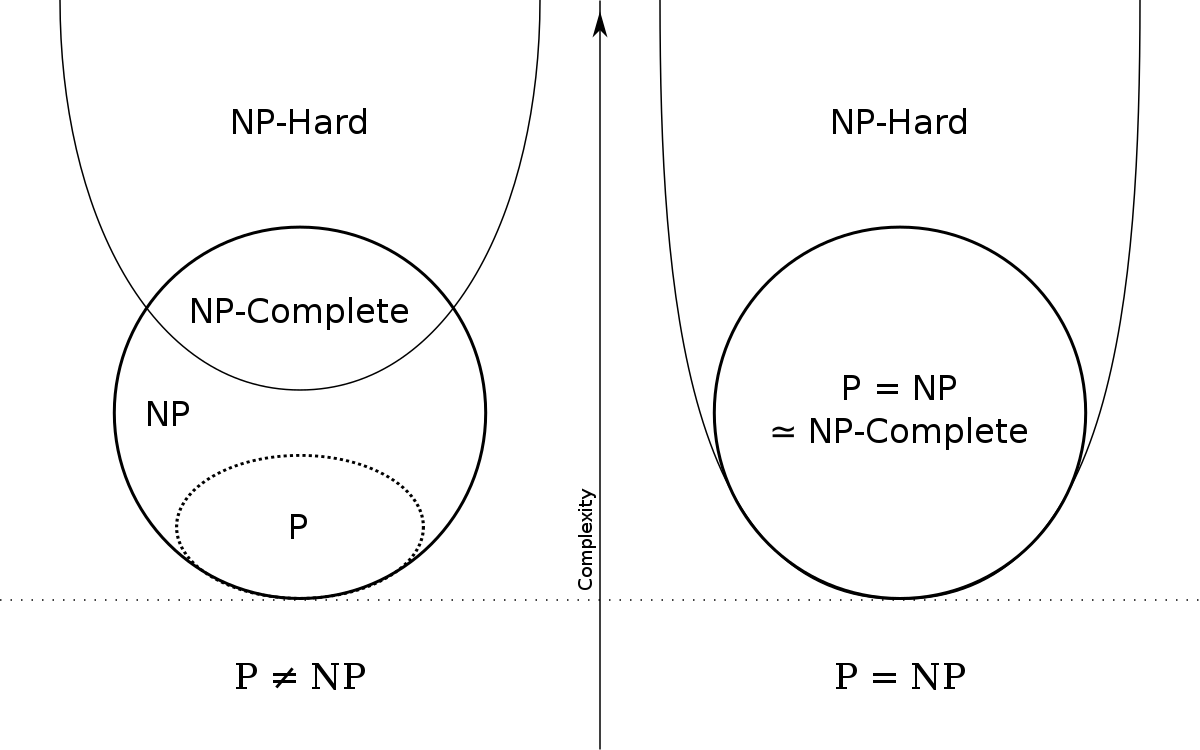
\includegraphics[scale = 0.3]{img/problem.png}
  \caption{Diagramma di \emph{Eulero Venn} per le classi di complessità}
  \label{fig:complexity}
\end{figure}
\begin{shaded}
  \textit{Tratto dagli appunti di Metodi Formali:}\\
\begin{center}
  \textit{Si parla di isomorfismo quando due strutture complesse si possono
    applicare l'una sull'altra, cioè far corrispondere l'una all'altra, in modo
    tale che per ogni parte di una delle strutture ci sia una parte
    corrispondente nell'altra struttura; in questo contesto diciamo che due
    parti sono corrispondenti se hanno un ruolo simile nelle rispettive
    strutture.}
\end{center}
Diamo ora una definizione formale di isomorfismo tra sistemi di transizione
etichettati, che possono quindi essere grafi dei casi o grafi dei casi
sequenziali.
\begin{definizione}
  Siano dati due sistemi di transizione etichettati:\\
  $A_1 = (S_1,E_1,T_1,s_{01})$ e $A_2 = (S_2 , E_2 , T_2 , s_{02})$.\\
  e siano date due \textbf{mappe biunivoche}:
  \begin{enumerate}
    \item $\alpha:S_1\to S_2$, ovvero che passa dagli stati del primo sistema a
    quelli del secondo
    \item $\beta:E_1\to E_2$, ovvero che passa dagli eventi del primo sistema a
    quelli del secondo
  \end{enumerate}
  allora:
  \[\langle \alpha,\beta\rangle:A_1= (S_1 , E_1 , T_1 ,s_{01})\to A_2 = (S_2 ,
    E_2 , T_2 , s_{02})\]
  è un \textbf{isomorfismo} sse:
  \begin{itemize}
    \item $\alpha(s_{01})=s_{02}$, ovvero l'immagine dello stato iniziale del
    primo sistema coincide con lo stato iniziale del secondo
    \item $\forall s,s'\in S_1,\forall e\in E_1:\,(s,e,s')\in T_1
    \Leftrightarrow (\alpha(s),\beta(e),\alpha(s'))\in T_2$ ovvero per ogni
    coppia di stati del primo sistema, tra cui esiste un arco etichettato $e$,
    vale che esiste un arco, etichettato con l'immagine di $e$, nel secondo
    sistema che va dall'immagine del primo stato considerato del primo sistema
    all'immagine del secondo stato considerato del secondo sistema, e viceversa
  \end{itemize}
\end{definizione}
\begin{definizione}
  Si definiscono due \textbf{sistemi equivalenti} sse hanno grafi dei casi
  sequenziali, e quindi di conseguenza anche grafi dei casi, \emph{isomorfi}.\\
  Due sistemi equivalenti accettano ed eseguono le stesse sequenze di eventi
\end{definizione}
\end{shaded}
\section{Riduzioni polinomiali}
Si hanno alcuni problemi che sono in grado di risolvere qualunque problema di
decisione in \textbf{NP}. Serviranno prima le definizioni di \textbf{NP-hard} e
\textbf{NP-complete}.\\
Vediamo innanzitutto il problema \textit{independent-set} che ci aiuterà
analisi.
\begin{definizione}
  L'\textit{independent-set } di un grafo non orientato è un sottoinsieme
  $I\subseteq V$ tale che $\forall u,v\in I$ $(u,v)\not\in E$. Il problema
  \textit{ind\_set}, nella versione di ottimo, è quello di trovare
  l'\textit{independent-set} di cardinalità massima di un grafo non
  orientato. Nella versione di decisione $ind\_set_d$ si ha anche il parametro
  $k$ intero e si cerca se esiste un \textit{independent-set} di cardinalità
  uguale a $k$. L'\textit{independent-set} di cardinalità massima può essere
  usato come ``certificato''.
\end{definizione}
Questo problema è legato alla \textit{copertura dei vertici}, infatti sappiamo
che se dall'insieme dei vertici togliamo un sottoinsieme di minima copertura
troviamo un \textit{independent-set} di cardinalità massima perché sto facendo
il complemento di un insieme di copertura di cardinalità minima, infatti tra i
vertici non nell'insieme di copertura di cardinalità minima, ovvero nel
complemento, non posso avere un arco per definizione e quindi se il primo è di
cardinalità minima allora il secondo, che è l'\textit{independent-set}, è di
cardinalità massima. Infatti i vertici nella copertura sono vertici che toccano
tutti gli archi.\\
Dal punto di vista delle applicazioni pratiche questi problemi si prestano allo
studio, per esempio, delle telecomunicazioni.
\begin{proof}
  Dimostriamo che $ind\_set_d$ è \textbf{NP}, infatti esiste un algoritmo $A$
  che in costo polinomiale prende in ingresso il grafo, $k$, e un
  ``certificato'' $y$ e i vertici in $y$, che sono vertici di un
  \textit{independent\_set} per il grafo $G$ di cardinalità $k$. L'algoritmo
  verifica che $y$ è un \textit{independent-set} e il costo della verifica è
  quadratico su $|y|$, ovvero $|y|^2$ che nel caso peggiore è $|V|^2$. So anche
  che, per l'input $x$, $O(|x|)=O(|E|+|V|)=O(|V^2|+|V|)$ nel caso peggiore,
  quindi il tempo di verifica è \textbf{polinomiale}.
\end{proof}
\begin{definizione}
  Vediamo ora il problema di \textbf{soddisfacibilità} $SAT$. Questo problema
  prende in input una formula booleana $\phi$ in \textbf{forma normale congiunta
    (CNF)}, ovvero che ha una congiunzione ($\lan$d) come legame tra le
  \textbf{clausole}. Una clausola è un $\lor$ di \textbf{letterali}, ovvero di
  variabili booleane $x_i$ o $\neg x_i$. In output ho se la forma sia
  soddisfacibile o meno. 
  \begin{esempio}
    Prendo 3 variabili, $x_1,x_2,x_3$. Creo i letterali  $x_1,x_2,x_3$ e anche
    $\neg x_1,\neg x_2,\neg x_3$. Creo quindi le clausole $c_1=x_1\lor x_2$,
    $c_2=x_1\lor \neg x_2$ e $c_3=x_1\lor \neg x_2$. Definisco quindi la CNF
    $\phi$:
    
    \[\phi=(x_1\lor x_2)\land (x_1\lor \neg x_2)\land
      (x_1\lor \neg x_2)=c_1\land c_2\land c_3\]
    Quindi in ogni clausola almeno un letterale deve essere vero, cosicché tutte
    le clausole siano vere rendendo vera la CNF.\\
    Avendo due letterali a clausola si è definito un $2SAT$.
  \end{esempio}
  Il numero di letterali $k$ che compongono la clausola definsice un problema
  $kSAT$. Si ha che $2SAT\in P$ ma con $k>2$ si ha che $kSAT\in NP$ (in
  realtà è in \textbf{NP-hard})
\end{definizione}
\begin{definizione}
  Definiamo un problema \textbf{NP-hard} come un problema difficile almeno
  quanto un problema \textbf{NP}. Ogni che problema $A$ in \textbf{NP} può
  essere risolto con un chiamata di procedura a $B$, che è un problema
  \textbf{NP-hard} a cui tutti gli altri ``chiedono aiuto'' per trovare una
  soluzione. \\
  Ad esempio \textit{vertex-cover} è un problema \textbf{NP-hard} e quindi posso
  risolvere ogni problema $A$ in \textbf{NP} con il problema
  \textit{vertex-cover} $B$.\\
  Trasformo quindi l'input $w$ di $A$ in un input
  $f(w)$ per $B$ in tempo polinomiale. La risposta di $B$ con input $f(w)$ è la
  stessa che $A$ da su input $w$.\\
  Non tutti i problemi \textbf{NP-hard} sono dentro la classe \textbf{NP}
\end{definizione}
\begin{definizione}
  Definiamo quindi il concetto di \textbf{riduzione}, rappresentato in figura
  \ref{fig:rid}.\\
  La riduzione è la trasformazione dell'input di $w$ in $A$ in un input $f(w)$
  per $B$, in tempo polinomiale. La risposta di $B$ con input $f(w)$ è la stessa
  che $A$ da su input $w$.\\
  Si ha che $A$ si riduce polinomialmente a $B$, e si scrive:
  \[A\leq_p B\]
  se $\exists\,f$ tale che:
  \[w \in L_A\mbox{ sse } f(w)\in L_B\]
  con $f$ calcolabile in tempo polinomiale, infatti il calcolo di $f(w)$ è
  $=(|w|^p)$, con $p\in\mathbb{N}$ per semplicità. Non devo introdurre una
  complessità superiore nel contesto di confronto tra problemi (??).\\ 
  \begin{figure}
    \centering
    
    \psscalebox{0.9 0.9} % Change this value to rescale the drawing.
    {
      \begin{pspicture}(0,-2.8)(15.0,2.8)
        \definecolor{colour1}{rgb}{0.34901962,0.6627451,0.3019608}
        \definecolor{colour0}{rgb}{0.8784314,0.20392157,0.20392157}
        \definecolor{colour2}{rgb}{0.3254902,0.38039216,0.99607843}
        \psframe[linecolor=colour1, linewidth=0.04, dimen=outer]
        (13.52,2.8)(1.52,-2.8)
        \psframe[linecolor=colour0, linewidth=0.04, dimen=outer]
        (6.32,1.2)(2.72,-1.2)
        \psframe[linecolor=colour0, linewidth=0.04, dimen=outer]
        (6.32,1.2)(2.72,-1.2)
        \psframe[linecolor=colour2, linewidth=0.04, dimen=outer]
        (11.52,1.2)(7.92,-1.2)
        \psline[linecolor=black, linewidth=0.04, arrowsize=0.05291667cm 2.0,
        arrowlength=1.4,arrowinset=0.0]{->}(6.32,0.0)(7.92,0.0)
        \psline[linecolor=black, linewidth=0.04, arrowsize=0.05291667cm 2.0,
        arrowlength=1.4,arrowinset=0.0]{->}(0.72,0.0)(2.72,0.0)
        \psline[linecolor=black, linewidth=0.04, arrowsize=0.05291667cm 2.0,
        arrowlength=1.4,arrowinset=0.0]{->}(11.52,0.4)(14.32,0.4)
        \psline[linecolor=black, linewidth=0.04, arrowsize=0.05291667cm 2.0,
        arrowlength=1.4,arrowinset=0.0]{->}(11.52,-0.4)(14.32,-0.4)
        \rput[bl](3.7,1.3){Riduzione}
        \rput[bl](0.0,-0.14){$w$}
        \rput[bl](4.1,-0.08){$f(w)$}
        \rput[bl](9.42,-0.08){$B$}
        \rput[bl](12.26,0.6){yes}
        \rput[bl](14.42,0.25){yes}
        \rput[bl](12.34,-0.74){no}
        \rput[bl](14.42,-0.5){no}
        \rput[bl](9.24,1.3){$SAT$}
        \rput[bl](6.72,0.4){$f(w)$}
      \end{pspicture}
    }
    \caption{Rappresentazione grafica della riduzione}
    \label{fig:rid}
  \end{figure}
  Ogni problema $A$ che in \textbf{NP} può essere risolto con una chiamata di
  procedura a $B$, quindi posso risolvere ogni problema $A\in NP$ con
  \textit{vertex-cover}, essendo esso un problema \textbf{NP-hard}.
  
\end{definizione}
\begin{definizione}
  $B$ è \textbf{NP-hard} sse $\for A\in NP$ $A$ si riduce a $B$ in tempo
  polinomiale:
  \[A\leq_p B,\,\,\forall A\]
  Un problema $NP-hard$ può non essere in $NP$, in quanto potrebbe non avere un
  ``certificato'' per consentire la verifica in tempo polinomiale.
\end{definizione}
\begin{definizione}
  Un problema \textbf{NP-hard} e anche \textbf{NP} si dice che il problema è
  \textbf{NP-complete} 
\end{definizione}
$kSAT$ è il primo problema che si è dimostrato essere anche
\textbf{NP-complete}.
\begin{esempio}
  Vediamo un esempio di riduzione, rappresentata in figura \ref{fig:ride}:
  \[3SAT\leq_p ind\_set_d\]
  arrivando e alla conclusione che $ind\_set_d$ è \textbf{NP-completo}.\\
  \begin{figure}
    \centering
    
    \psscalebox{0.9 0.9} % Change this value to rescale the drawing.
    {
      \begin{pspicture}(0,-2.8)(15.0,2.8)
        \definecolor{colour1}{rgb}{0.34901962,0.6627451,0.3019608}
        \definecolor{colour0}{rgb}{0.8784314,0.20392157,0.20392157}
        \definecolor{colour2}{rgb}{0.3254902,0.38039216,0.99607843}
        \psframe[linecolor=colour1, linewidth=0.04, dimen=outer]
        (13.52,2.8)(1.52,-2.8)
        \psframe[linecolor=colour0, linewidth=0.04, dimen=outer]
        (6.32,1.2)(2.72,-1.2)
        \psframe[linecolor=colour0, linewidth=0.04, dimen=outer]
        (6.32,1.2)(2.72,-1.2)
        \psframe[linecolor=colour2, linewidth=0.04, dimen=outer]
        (11.52,1.2)(7.92,-1.2)
        \psline[linecolor=black, linewidth=0.04, arrowsize=0.05291667cm 2.0,
        arrowlength=1.4,arrowinset=0.0]{->}(6.32,0.0)(7.92,0.0)
        \psline[linecolor=black, linewidth=0.04, arrowsize=0.05291667cm 2.0,
        arrowlength=1.4,arrowinset=0.0]{->}(0.72,0.0)(2.72,0.0)
        \psline[linecolor=black, linewidth=0.04, arrowsize=0.05291667cm 2.0,
        arrowlength=1.4,arrowinset=0.0]{->}(11.52,0.4)(14.32,0.4)
        \psline[linecolor=black, linewidth=0.04, arrowsize=0.05291667cm 2.0,
        arrowlength=1.4,arrowinset=0.0]{->}(11.52,-0.4)(14.32,-0.4)
        \rput[bl](3.7,1.3){Riduzione}
        \rput[bl](0.35,-0.15){$\phi$}
        \rput[bl](4.1,-0.08){$f(\phi)$}
        \rput[bl](9.42,-0.08){$B$}
        \rput[bl](14.42,0.25){1}
        \rput[bl](14.42,-0.5){0}
        \rput[bl](9.0,1.3){$ind\_set_d$}
        \rput[bl](6.85,0.2){$G_\phi$}
      \end{pspicture}
    }
    \caption{Rappresentazione grafica del'esempio \ref{es:1}}
    \label{fig:ride}
  \end{figure}
  e vediamo che $\phi$ è soddisfacibile sse $G_\phi$ ha un
  \textit{independent-set} di dimensione $k=|\phi|$, con $|\phi|$ pari al numero
  di clausole della formula.\\
  Costruisco quindi un grafo che ha un vertice per ogni letterale della
  clausola. Collego i tre letterale della clausola ottenendo un
  ``triangolo'', detto \textit{gadget}, che rappresenta una clausola. Infine
  collego ogni letterale al suo negato.
  \newpage
  Quindi per la formula:
  \[\phi=(\neg x_1\lor x_2\lor x_3)\land(x_1\lor \neg x_2\lor x_3)\land(\neg
    x_1\lor x_2\lor x_4)\]
  avrò il grafo $G_\phi$ che codifica la formula $\phi$:
  \begin{figure}[H]
    \centering
    \psscalebox{1.0 1.0} % Change this value to rescale the drawing.
    {
      \begin{pspicture}(0,-1.5798438)(12.92,1.5798438)
        \pscircle[linecolor=black, linewidth=0.04, fillstyle=solid,
        fillcolor=black, dimen=outer](1.6,0.9050586){0.4}
        \pscircle[linecolor=black, linewidth=0.04, fillstyle=solid,
        fillcolor=black, dimen=outer](0.4,-0.6949414){0.4}
        \pscircle[linecolor=black, linewidth=0.04, fillstyle=solid,
        fillcolor=black, dimen=outer](2.8,-0.6949414){0.4}
        \psline[linecolor=black, linewidth=0.02](1.6,0.5050586)(2.4,-0.6949414)
        \psline[linecolor=black, linewidth=0.02](1.6,0.5050586)(0.8,-0.6949414)
        \psline[linecolor=black, linewidth=0.02](0.8,-0.6949414)(2.4,-0.6949414)
        \rput[bl](1.2,1.3050586){$\neg x_1$}
        \rput[bl](2.6,-1.4949414){$x_3$}
        \rput[bl](0.2,-1.4949414){$x_2$}
        \pscircle[linecolor=black, linewidth=0.04, fillstyle=solid,
        fillcolor=black, dimen=outer](6.4,0.9050586){0.4}
        \pscircle[linecolor=black, linewidth=0.04, fillstyle=solid,
        fillcolor=black, dimen=outer](5.2,-0.6949414){0.4}
        \pscircle[linecolor=black, linewidth=0.04, fillstyle=solid,
        fillcolor=black, dimen=outer](7.6,-0.6949414){0.4}
        \psline[linecolor=black, linewidth=0.02](6.4,0.5050586)(7.2,-0.6949414)
        \psline[linecolor=black, linewidth=0.02](6.4,0.5050586)(5.6,-0.6949414)
        \psline[linecolor=black, linewidth=0.02](5.6,-0.6949414)(7.2,-0.6949414)
        \rput[bl](6,1.3050586){$\neg x_2$}
        \rput[bl](7.4,-1.4949414){$x_3$}
        \rput[bl](5.0,-1.4949414){$x_1$}
        \pscircle[linecolor=black, linewidth=0.04, fillstyle=solid,
        fillcolor=black, dimen=outer](11.2,0.9050586){0.4}
        \pscircle[linecolor=black, linewidth=0.04, fillstyle=solid,
        fillcolor=black, dimen=outer](10.0,-0.6949414){0.4}
        \pscircle[linecolor=black, linewidth=0.04, fillstyle=solid,
        fillcolor=black, dimen=outer](12.4,-0.6949414){0.4}
        \psline[linecolor=black,linewidth=0.02](11.2,0.5050586)(12.0,-0.6949414)
        \psline[linecolor=black,linewidth=0.02](11.2,0.5050586)(10.4,-0.6949414)
        \psline[linecolor=black,linewidth=0.02]
        (10.4,-0.6949414)(12.0,-0.6949414)
        \rput[bl](10.8,1.3050586){$\neg x_1$}
        \rput[bl](12.2,-1.4949414){$x_4$}
        \rput[bl](9.8,-1.4949414){$x_2$}
        \psline[linecolor=black, linewidth=0.02](0.8,-0.6949414)(6.0,0.9050586)
        \psline[linecolor=black, linewidth=0.02](2.0,0.9050586)(4.8,-0.6949414)
        \psline[linecolor=black, linewidth=0.02](5.6,-0.6949414)(10.8,0.9050586)
        \psline[linecolor=black, linewidth=0.02](6.8,0.9050586)(9.6,-0.6949414)
      \end{pspicture}
    }
    \label{es:1}
  \end{figure}
  Quindi un \textbf{gadget} è una rappresentazione dell'input del problema $A$
  di partenza e ogni \textbf{gadget} rappresenta una clausola.\\
  Ricordiamo che $\phi$ è soddisfacibile sse esiste un assegnamento delle
  variabili della formula tale per cui almeno un letterale di ogni clausola è
  vero. Nel grafo relativo alla formula lego quindi un letterale ad ogni suo
  complemento al fine di poter identificare i valori di verità e avendo il
  calcolo di \textit{independent-set} (per la \textbf{riduzione}) prendo uno
  solo degli estremi di un arco, e quindi uno solo tra $x_i$ e $\neg x_i$,
  codificando l'assegnamento di verità. Il concetto di \textbf{riduzione} è
  quindi ritrovabile nella capacità di rappresentare un problema in un'altra
  forma, studiabile con un altro algoritmo.
  \begin{proof}
    Indichiamo con $A$ $3SAT$ e con $B$ \textit{independent-set}.\\
    Effettuiamo quindi la prova finale, la dimostrazione vera e propria. A
    questo livello di comprensione abbiamo dimostrato
    l'esistenza della funzione $f$, che trasforma $\phi$ (ovvero l'input di $A$)
    in $\langle G, k\rangle$, ovvero l'input di $B$, e che essa è in tempo
    polinomiale. Abbiamo quindi che $w\in L_A$ sse $f(w)\in L_B$. Se $\phi$ è
    vera allora esiste un \textit{independent-set} di dimensione $k$ per
    $\langle G, k\rangle$.\\ 
    Nell'\,''altro verso'' abbiamo che se esiste un \textit{independent-set} di
    dimensione $k$ per $\langle G, k\rangle$ allora $\phi$ è vera. Dimostrare
    questi due ``versi'' equivale a dimostrare la riduzione.\\
    Il \textbf{primo verso} si dimostra dicendo che dato un assegnamento di
    verità si seleziona un letterale vero da ogni triangolo. Questi letterali
    veri scelti formano l'\textit{independent-set} $S$, che ha dimensione
    $k$. Questo può accadere sse $\phi$ è vera, infatti per ogni clausola $c_i$
    $\exists \,\,l_{ij}$, letterale, che rende vera $c_i$, a questo punto tale
    letterale è un vertice del triangolo, ovvero del gadget $g_{c_i}$, (mi basta
    infatti un letterale vero per triangolo) e, poiché
    tutte le clausole sono vere, ho la scelta di $k$ vertici se $k$ è il numero
    delle clausole. Esiste quindi un \textit{independent-set} di dimensione
    $k$.\\
    Per questo si potrebbe fare una \textbf{dimostrazione per costruzione},
    ovvero se rendo vera $c_y$ con $l_y$ significa che la variabile $x_i$ può
    essere usata o come 1 o come 0 nell'assegnamento di verità in un altro
    letterale $l_z$, che rende vera la clausola $c_z$. Ma $x_i$, se già usata,
    non posso più usarla con valore opposto a quello scelto per $c_y$ e quindi
    non esiste un arco di collegamento tra $l_y$ e $l_z$.\\
    Si può dimostrare anche per \textbf{assurdo}. Se esiste un arco tra i due
    letterali $l_z$ e $l_y$ che rendono vere le clausole $c_z$ e $c_y$,
    allora ottengo una contraddizione sugli assegnamenti di verità, asserendo
    che i due letterali sono uno la negazione dell'altro ma entrambi sono
    veri, per poter rendere vere le clausole. 
    \\
    \\
    Il \textbf{secondo verso} si dimostra dicendo che, dato un
    \textit{independent-set} 
    $S$ di dimensione $k$, $S$ deve contenere un vertice per triangolo. Ponendo
    quindi i letterali contenuti in $S$ come veri si ottiene un assegnamento di
    verità che è \textbf{consistente} e tutte le clausole sono soddisfatte.
    Quindi se esiste un \textit{independent-set} di dimensione $k$ allora trovo
    un assegnamento alle variabili $x_i,\,\,\forall \,\,1\ldots n$ che rende
    vera $\phi$, ovvero assegno 0 o 1 a ciascuna variabile (ovviamente o 1 o 0,
    non entrambi). Se esiste l'\textit{independent-set} di dimensione $k$ pari
    al numero delle clausole, allora per ogni gadget $g_{c_i}$,
    che rappresenta una clausola, esiste un vertice nel gadget che si trova
    anche nell'\textit{independent-set}, quindi esiste un letterale, per ogni
    clausola $c_i$ tale che non è collegato ad un altro letterale
    dell'\textit{independent-set}, ovvero non è collegato ad un altro letterale
    di un'altra clausola (ovvero ho un nodo per gadget che non ha un arco verso
    un nodo di un altro gadget). Quindi per ogni letterale vedo la variabile che
    rende vero il letterale e con il valore dato alla variabile costruisco
    l'assegnamento o 0 o 1 a quella variabile (se $l_i=\neg x_j$ allora
    $x_j=0$ e se $l_i= x_j$ allora $x_j=1$). Trovo quindi l'assegnamento delle
    variabili che è di verità per $\phi$, dimostrando quindi che $\phi$ è vera.
  \end{proof}
\end{esempio}
Siccome $3SAT$ è \textbf{NP-complete} allora anche \textit{independent-set} è
\textbf{NP-complete}, infatti:
\[\forall\,\, A_{\in NP}\leq_p 3SAT\leq_p \mbox{ \textit{independent-set}}\]
in quanto la riduzione $\leq_p$ è \textbf{transitiva}, e quindi:
\[\forall\,\, A_{\in NP}\leq_p \mbox{ \textit{independent-set}}\in NP\]
\begin{teorema}
  Se un problema $\Pi$ \textbf{NP-complete} è in \textbf{P} allora si può dire
  $P=NP$, implicando che ogni problema $A\in NP$ è risolvibile da $\Pi\in P$.
  Questa cosa non è stata ancora dimostrata (e probabilmente si riuscirà
  a dimostrare l'opposto).
\end{teorema}
\begin{proof}
  Per ogni problema $A$ in \textbf{NP} so che $A\leq_p \Pi$, ovvero $\Pi$ è una
  procedura che risolve $A$, con trasformazione dell'input $x$ di $A$ nell'input
  $f(x)$ di $\Pi$, con $f(x)$ calcolabile in tempo polinomiale.\\
  Assumendo quindi che $\Pi\in P$ allora anche ogni $A\in P$, e quindi $NP=P$.
\end{proof}
\begin{teorema}
  La riduzione polinomiale è transitiva. Ovvero se $A\leq_p B$ e $B\leq_p C$
  allora:
  \[A\leq_p C\]
\end{teorema}
\begin{proof}
  Infatti $A\leq_p B$ implica l'esistenza di $f$ tale che $x\in L_A$ sse
  $f(x)=L_B$. Ugualmente $B\leq_p C$ implica l'esistenza di $g$ tale che $x\in
  L_B$ sse $g(x)=L_C$.\\
  Devo dimostrare che $\exists\,\,f'$ tale che $x\in L_A$ sse $f'(x)\in
  L_C$. Per ottenere $f'$ compongo $f$ e $g$. Assumendo che $x$ appartiene
  all'input di ha compongo le funzioni, quindi ho che $f'=g\circ f$,
  e ho che $x\in L_A$ e che $f(x)\in L_B$ (quindi $f(x)$ è un input per $B$) ma
  quindi $g(f(x))\in L_C$ (quindi $g(f(x))$ è un input per $C$). Ho quindi
  dimostrato la transitività.\\
  Se $f$ e $g$ sono costruibili in tempo polinomiale, la prima sulla dimensione
  di $x$ e la seconda su quella di $f(x)$, allora anche $f'=g\circ f$
  è costruibile in tempo polinomiale, proporzionalmente alla cardinalità di $x$.
\end{proof}
Quindi per dimostrare che un problema $\Pi'$ è \textbf{NP-hard} devo ridurre
$\Pi'$ ad un problema qualsiasi \textbf{NP-hard} (in base alla somiglianza del
problema), sapendo che $\forall A\in NP$ $A$ si riduce ad un problema
\textbf{NP-hard}, come $SAT$.\\
In modo equivalente per dire che è un problema è \textbf{NP-complete} faccio
quanto fatto per \textbf{NP-hard} ma devo aggiungere che esso sia in $NP$,
dovendo quindi aggiungere il ``certificato''.
% immagine slide 6(teorema cook)
\begin{teorema}
  Si ha che $SAT\leq_p 3SAT$
\end{teorema}
\begin{proof}
  \textbf{Dimostrazione solo parziale, solo l'inizio è stato fatto in aula.\\}
  Prendo una $\phi$ con $k\geq 4$ letterali. Ogni clausola deve diventare una
  clausola con al più 3 letterali (introducendo nuovi letterali ogni volta che
  viene negato uno). 
\end{proof}
\subsection{Problema set-cover}
Questo problema si applica bene allo studio, nel campo delle telecomunicazioni,
dei ripetitori e dello studio della copertura per reti mobili.
\begin{definizione}
  Dato un universo $U$ di $n$ elementi sia $S=\{S_1,\ldots,S_M\}$ una collezione
  di sottoinsiemi di $U$. Sia anche data una funzione di costo
  $c:S\to\mathbb{Q}^+$. Il problema \textbf{set-cover} consiste nel trovare una
  collezione $C$ di sottoinsiemi di $S$ di costo minimo che copra tutti gli
  elementi di $U$.
\end{definizione}
\begin{esempio}
  Se ho $U=\{1,2,3,4,5\}$, $S_1=\{1,2,3\}$, $S_2=\{2,3\}$, $S_3=\{4,5\}$ e
  $S_4=\{1,2,4\}$, con $S=\bigcup S_i$ . Per praticità assumo costo
  uniforme, ovvero che  $c_1=c_2=c_3=c_4=1$.\\
  Quindi la soluzione $C$ è $\{S_1,S_3\}$, in quanto questi due insiemi coprono
  tutti gli elementi di $U$, con costo pari a $5$ (che è il minimo che posso
  avere).
\end{esempio}
\begin{definizione}
  Qualora il costo sia uniforme allora il \textbf{set-cover} diventa la ricerca
  di una sotto-collezione che copra tutti gli elementi di $U$ con minima
  dimensione.
\end{definizione}

\begin{teorema}
  \textit{set-cover}, nella versione decisionale e nella
  versione con peso uniforme, è \textbf{NP-complete} (quindi se esiste una
  collezione $C$ di sottoinsiemi di $S$ 
  la cui unione sia $U$ con cardinalità minore uguale di $k$).
\end{teorema}
\begin{proof}
  Posso facilmente dimostrare che $|C|\leq k$ in tempo polinomiale e che
  l'unione degli insieme di $C$ include tutti gli elementi di $U$, in
  tempo polinomiale su $|U|$. Posso aggiungere anche un ``certificato'', nella
  forma di una collezione che copre tutto $U$ (e quindi la verifica è in tempo
  polinomiale sulla dimensione del ``certificato'' più quella di $U$). Quindi
  \textbf{set-cover} è in \textbf{NP}.\\
  Per dimostrare che \textbf{set-cover} è \textbf{NP-hard} dimostro che:
  \[\mbox{vertex-cover} \leq_p \mbox{set-cover}\]
  ovvero uso un problema che so già essere \textbf{NP-hard}, appunto
  \textit{vertex-cover} (avendo già dimostrato che $\forall A\in NP, \,\,A\leq_p
  \mbox{vertex-cover}$, dimostrando che \textit{set-cover} dimostra tutti i
  problemi in \textbf{NP}).\\
  Faccio vedere che posso usare \textit{set-cover} per dimostrare
  \textit{vertex-cover}.\\
  Devo quindi trasformare un'istanza di \textit{vertex-cover} $C=\langle
  G=(V,E), j\rangle$ in un'istanza $C'$ di \textit{set-cover}, in tempo
  polinomiale, tale che $C$ è soddisfacibile sse $C'$ è soddisfacibile.\\
  Procedo quindi con la trasformazione. Pongo innanzitutto $U=E$. Per quanto
  riguarda la collezione $S$ procedo nel seguente modo. Etichetto i vertici in
  $V$ da $1$ a $n$. A questo punto $S_i$ diventa l'insieme degli archi incidenti
  al vertice $i$-simo. A questo punto basta porre $k=j$ per concludere la
  costruzione polinomiale dell'istanza di \textit{set-cover}.\\
  In poche parole ciascun arco è un elemento di $U$ e ciascun vertice è un
  insieme di $S$.\\
  Vediamo anche la dimostrazione formale che \textit{vertex-cover} risponde
  ``yes'', per $j$, sse istanza di \textit{set-cover} risponde ``yes'' per
  $k=j$.\\
  Innanzitutto se \textit{vertex-cover} risponde ``yes'' per $j$ allora trovo
  una collezione di \textit{set-cover} buona di cardinalità $j$. Suppongo
  infatti $G$ ha una copertura C di al più $j$ vertici e quindi $C$ corrisponde
  ad una collezione di $C'$ di sottoinsiemi $U$. Poiché assumo $k=j$ allora
  $|C'|\leq k$. Inoltre $C'$ copre tutti gli elementi di $U$ coprendo tutti gli
  archi di $G$, in quanto ogni elemento di $U$ è un arco in $G$. Poiché $C$ è
  una copertura, almeno un estremo dell’arco è in $C$  e quindi l’arco è in un
  insieme di $C'$.\\
  Dimostriamo anche l'altro verso della dimostrazione, ovvero devo garantire
  l'esistenza della copertura. Suppongo di avere un set cover $C'$ di dimensione
  $k$. Dato che ad ogni insieme di $C'$ ho associato un vertice in $G$ allora
  $|C|=|C'|\leq k=j$. Inoltre, $C$ è una copertura di $G$ poiché $C'$ è un
  set-cover, poiché, preso un arco $e$ ho che $e\in U$ e quindi $C'$ deve
  contenere almeno un insieme che contiene $e$ e tale insieme è quello che
  corrisponde ai nodi che sono estremi di $e$. Quindi $C$ deve contenere almeno
  un estremo di $e$. Quindi posso concludere dicendo che $C$ è copertura di $G$.
\end{proof}

\end{document}


% LocalWords:  Machine Learning NP TM yes sse Access pseudocodice store add TSP
% LocalWords:  load esguite dimostrabilmente primis Stirling NTDM vertex cover
% LocalWords:  exptime all img problem png independent ind nell CNF definsice
% LocalWords:  soddisfacibilità polinomialmente dell
